\section{UseCase}
\begin{figure}[ht] 
\begin{center}
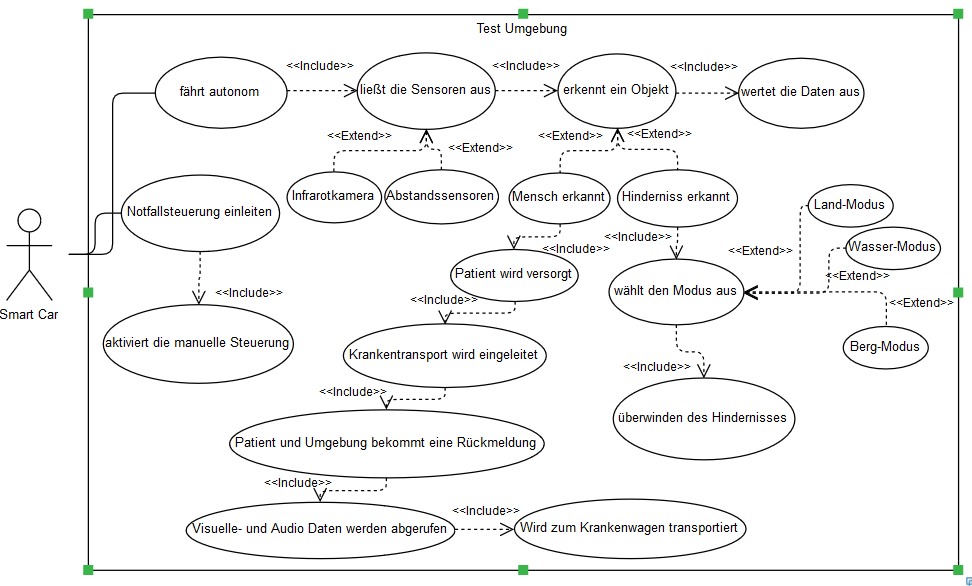
\includegraphics[width = 1\linewidth] {UseCase.png}
\caption{UseCase}
\end{center}
\end{figure}

Aus unseren Anforderungen haben wir ein Use Case Diagramm erstellt.
Wir recherchierten und stellten uns folgende Fragen:  
"Was wollen wir und was muss die Lösung des Projektes sein?"

Auf Fig.1. sieht man das erstellte Use Case Diagramm.
Zu sehen sind die drei Aktoren die als Mensch dargestellt werden.
Diese befinden sich außerhalb des Systems (Die Rettung eines Patienten).
Die Aktoren sind mit dem Use Cases verbunden.
Jeder Aktor hat unterschiedliche Aktivitäten wie, dass der Rescue Robot autonom fährt.
Die einzelnen Use Cases sind untereinander verbunden über include Beziehungen. 

Beispiel Ablauf:
Der Rescue Robot fährt autonom.
Dies included, dass ein Objekt erkannt wird.
Anschließend wird das Hindernis überwunden, indem zu der manuellen Steuerung gewechselt wird.
Daraufhin leitet der Aktor ''Operator'' den Krankentransport ein, versorgt den Patienten und gibt ihm Visuelle- und Audiodaten aus.
Zum Schluss folgt die Kommunikation zwischen dem Aktor ''Operator'' und dem Aktor ''Patienten.''

\subsection{Aktivitätsdiagramm}
Für jedes Use Case wurde daraufhin ein 
Aktivitätsdiagramm erstellt.
Beispiel ist Fig. 2. Hier zu sehen ist 
das Aktivitätsdiagramm des autonomen Fahren.
Das Diagramm beschreibt die Möglichkeiten vom autonomen Fahren.
Der Sensor wird ausgelesen, anschließend wird dann entschieden, 
ob der Rescu Robot links, rechts oder geradeaus lenkt.
Zum Schluss wird bestimmt, ob der Robot vorwärts oder rückwärts fährt.

\begin{figure}[ht] 
\begin{center}
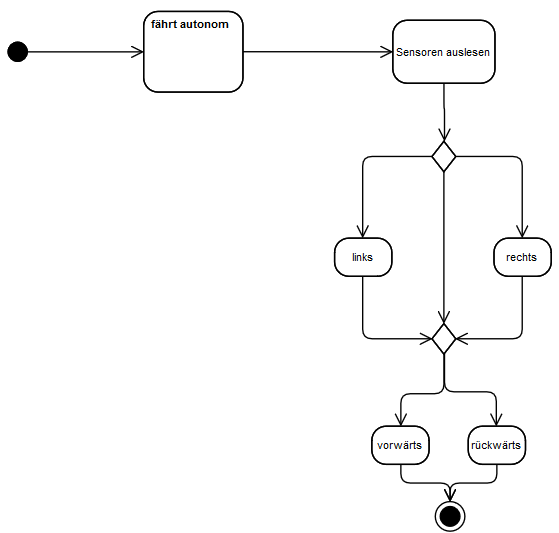
\includegraphics[width = 1\linewidth] {Aktiv.png}
\caption{Aktivitätsdiagramm}
\end{center}
\end{figure}